\chapter{Architettura}
\section{Approccio problema}
Si è deciso di approcciare il problema con una macchina a stati finiti. Trattandosi di un problema di complessità ridotta si è optato per una soluzione mono modulare con un singolo process che elabora i vari stati.

\section{Macchina a stati}
Di seguito una breve spiegazione degli stati della macchina e i segnali di controllo:
\begin{wrapfigure}{r}{0.50\textwidth}
    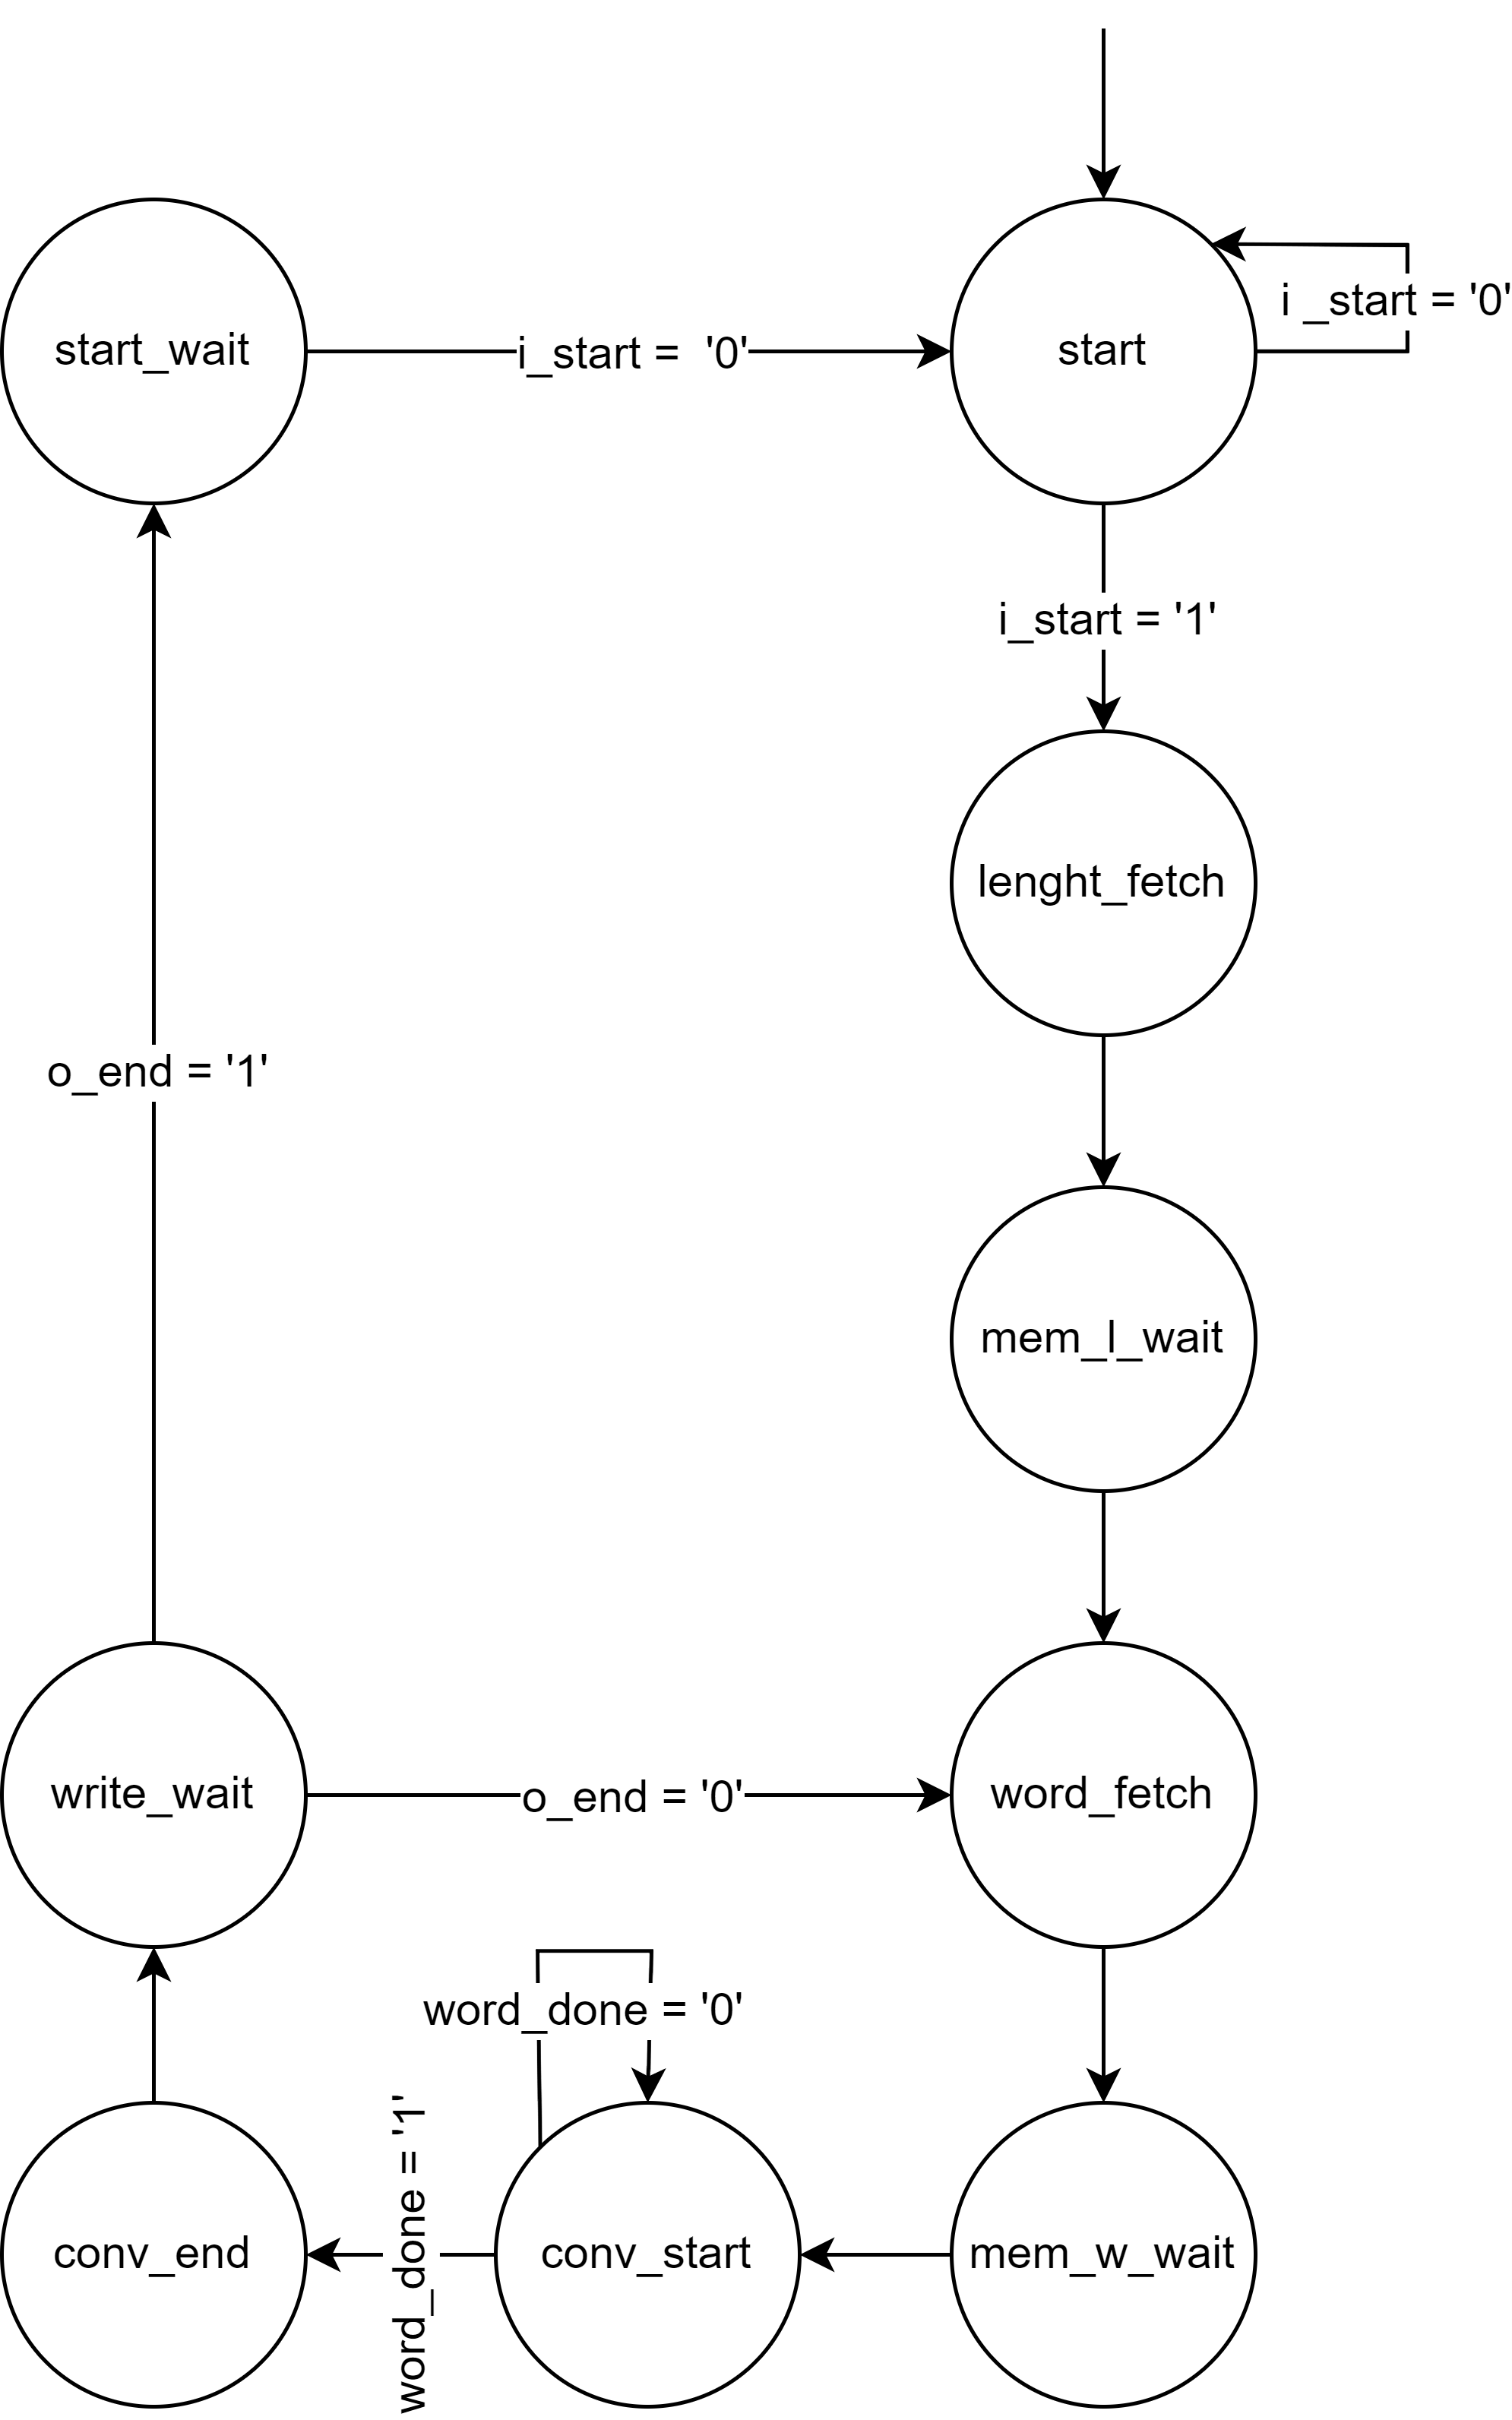
\includegraphics[trim=0cm 40cm 0cm 6.7cm, width=0.50\textwidth]{images/Capitolo2/vertical_fsm.png}
\end{wrapfigure}
\begin{itemize}
    \item \texttt{start}: Lo stato di inizio, è anche lo stato di reset. In questo stato si aspetta che il segnale \texttt{i\_start} venga alzato a 1.
    \item \texttt{length\_fetch}: Lo stato in cui vengono alzati i segnali per poter leggere dalla memoria, in particolare la lunghezza della parola.
    \item \texttt{mem\_l\_wait}: Lo stato di attesa per permettere alla memoria di caricare il dato.
    \item \texttt{word\_fetch}: Lo stato in cui vengono alzati i segnali per poter leggere dalla memoria, in particolare la parola.
    \item \texttt{mem\_w\_wait}: Lo stato di attesa per permettere alla memoria di caricare il dato.
\end{itemize}

\begin{itemize}
    \item \texttt{conv\_start}: Lo stato in cui viene eseguita la serializzazione e la codifica della parola. La macchina rimane in questo stato fino a quando \texttt{word\_done} viene posto a 1.
    \item \texttt{conv\_end}: Lo stato in cui la codifica è conclusa e inizia il processo di scrittura in memoria. (Primi Byte)
    \item \texttt{write\_wait}: Lo stato in cui termina il processo di scrittura in memoria (Secondo Byte).
    \item \texttt{start\_wait}: Lo stato di arrivo se la macchina ha codificato tutte le parole.
\end{itemize}

\section{Algoritmi implementati}
Di seguito una breve spiegazione della logica implementata per poter affrontare i problemi di serializzazione e parallelizzazione e di codifica delle parole.
\subsubsection{Serializzazione}
La serializzazione della parola si basa sull'utilizzo di shift. Infatti, quando necessario, viene salvato in un \texttt{std\_logic} il bit nella posizione più significativa della parola da codificare (che è salvata in un \texttt{std\_logic\_vector}); dopodiché al vettore viene effettuato uno shift una posizione verso sinistra, così che sia pronto per il prossimo ciclo.

\subsubsection{Codifica della parola} \label{codifica}
Supponendo che il bit da codificare sia chiamato \( msg \), i bit in output siano chiamati rispettivamente \( x_1 \) e \( x_0 \)\footnote{ \( x_1 \) è il bit più significativo rispetto a \( x_0 \)} e la bitmask dello stato corrente della macchina del convolutore siano rispettivamente \( m_1 \) e \( m_0 \)\footnote{ \( m_1 \) è il bit più significativo  rispetto a \( m_0 \)} allora è possibile constatare che:
\[ x_1 = msg \oplus m_0 \] \[ x_0 = msg \oplus m_1 \oplus m_0.\]
È anche possibile calcolare il prossimo stato della macchina del convolutore come:
\[ m_1 = msg\] \[ m_0 = x_1\]

\subsubsection{Parallelizzazione}
Dopo la codifica della parola si ha in uscita un flusso di bit. Anche la parallelizzazione del flusso si basa sull'utilizzo di shift, i bit in uscita (\texttt{std\_logic}) vengono salvati in un \texttt{std\_logic\_vector} in posizione 1 e 0 rispettivamente, dopo di che al vettore viene effettuato uno shift di una posizione verso sinistra, così che sia pronto per il prossimo ciclo.

\section{Registri Interni}
Di seguito una breve descrizione dei segnali interni per la gestione della logica.
\inputminted{vhdl}{listings/Capitolo2/signals.vhd}
\subsubsection{Counters}
\begin{itemize}
    \item \texttt{bit\_counter}: Tiene conto di quanti bit sono già stati codificati;
    \item \texttt{read\_address}: Tiene conto fino a che punto è stato scritto in memoria;
    \item \texttt{words\_read}: Tiene conto di quante parole sono state codificate.
\end{itemize}
\subsubsection{Flags}
\begin{itemize}
    \item \texttt{word\_done}: Viene settato a 1 se la parola è stata completamente codificata;
    \item \texttt{o\_end}: Viene settato a 1 se tutte le parole sono state codificate;
    \item \texttt{enable}: Viene settato a 1 quando inizia la codifica della parola.
\end{itemize}
\subsubsection{Useful signals}
\begin{itemize}
    \item \texttt{words\_to\_read}: Tiene conto di quante parole devono essere codificate;
    \item \texttt{word}: Contiene la parola da codificare;
    \item \texttt{message}: Contiene il bit della parola da codificare (utilizzato per: \ref{codifica});
    \item \texttt{merged}: Contiene il risultato della codifica della parola (utilizzato per: \ref{codifica}); 
    \item \texttt{state}: Rappresenta lo stato della macchina convoluzionale (utilizzato per: \ref{codifica}).
\end{itemize}

